\documentclass[12pt,a4paper]{article}

\usepackage[utf8]{inputenc}
\usepackage[ngerman]{babel}
\usepackage[T1]{fontenc}
\usepackage{amsmath}
\usepackage{amsfonts}
\usepackage{amssymb}
\usepackage{graphicx}
\usepackage[left=2cm,right=2cm,top=2cm,bottom=2cm]{geometry}
\usepackage{multicol}
\usepackage{booktabs}
\usepackage[hidelinks]{hyperref}
\usepackage{tikz}
\usepackage{pgfplots}
\usepackage{blindtext}
\usepackage{array}
\usepackage{multirow}
\usepackage{bigdelim}
\usepackage{colortbl}
\usepackage{fancyhdr} 
\usepackage{tabularx}
\usepackage{xcolor}
\usepackage{color}
\usetikzlibrary{decorations.text}
\usetikzlibrary{tikzmark}
\pagestyle{fancy} 
	\fancyhf{} 
	\fancyhead[L]{
\includegraphics[scale=0.05]{Bilder/dhbw.png}} 
	\fancyhead[C]{\slshape Formale Sprachen und Automaten} 
	\fancyhead[R]{\slshape LaTeX Version}
	\fancyfoot[C]{\thepage}
\usepackage{helvet}
\renewcommand{\familydefault}{\sfdefault}

\title{Formale Sprachen und Automaten}
\author{\slshape Robin Rausch, Florian Maslowski}
\date{\slshape \today}
\begin{document}
\pagenumbering{Roman}
\maketitle
\tableofcontents
\newpage
\pagenumbering{arabic}
\section{Grundlagen}
	\subsection{Alphabet}
	Ein Alphabet $\varSigma$ ist eine nicht-leere Menge von Symbolen(Zeichen, Buchstaben).
	Beispiel: $\varSigma_{ab} = { a, b }$

	\subsection{Wort}
	Ein Wort $w$ über dem Alphabet $\varSigma$(Sigma) ist eine endliche Folge von Symbolen aus $\varSigma$. Das Wort $w = abaabab$ wurde beispielsweise aus dem Alphabet $\varSigma_{ab}$ gebildet.\newline
	Die Länge eines Wortes kann durch Betragsstriche angegeben werden. Beispiel: $|w| = 7$\newline
	Ebenso kann man die Anzahl bestimmter Symbole in einem Wort bestimmen: $|w|_b = 3$\newline
	Ein einzelnes Zeichen kann durch eckige Klammern angegeben werden: $w[2] = b$\newline
	Wörter können bliebig konkateniert werden(hintereinanderschreiben ohne abstand): $w_1w_2 = abbabaab$ mit $w_1 = abba$ und $w_2 = baab$.\newline
	Wörter dürfen auch potenziert werden: $w^3 = abaabababaabababaabab = www$\newline
	Das leere Wort lautet $\varepsilon$.

	\subsection{Formale Sprachen}
	Eine formale Sprache $L$ über einem Alphabet $\varSigma$ ist eine Menge von Wörtern aus $\varSigma^*: L \subseteq \varSigma^*$. Eine Sprache kann sowohl endlich als auch unendlich sein.\newline
	Beispiel: $L_1 = \{w \in \varSigma_{bin}^* |$ $|w| \geqslant 2 \wedge w[|w| - 1] = 1\}$ ist die Menge aller Binärwörter, an deren vorletzter Stelle 1 steht.\newline
	Das Produkt zweier formaler Sprachen: $L_1 \cdot L_2 = \{abac, abcb, bcac, bccb\}$ mit $L_1 = \{ab, bc\}$ und $L_2 = \{ ac, cb\}$.\newline
	Sprachen können ebenfalls potenziert werden: $L^2 = \{ab, ba\} \cdot \{ab, ba\} = \{ abab, abba, baab, baba\}$

	\subsection{Kleene Stern}
	Für ein Alphabet $\varSigma$ und eine formale Sprache $L \subseteq \varSigma^*$ ist der Operator Kleene Stern wie folgt definiert: $L^* = \underset{n \in \mathbb{N}}{\bigcup} L^n$.\newline \newline
	Beispiel: Sei $L_1 = \{ ab, ba\}$, dann $L^* = \{\varepsilon, ab, ba, abab, abba, baab, baba, ababab, ...\}$.

	\subsection{Überblick}
	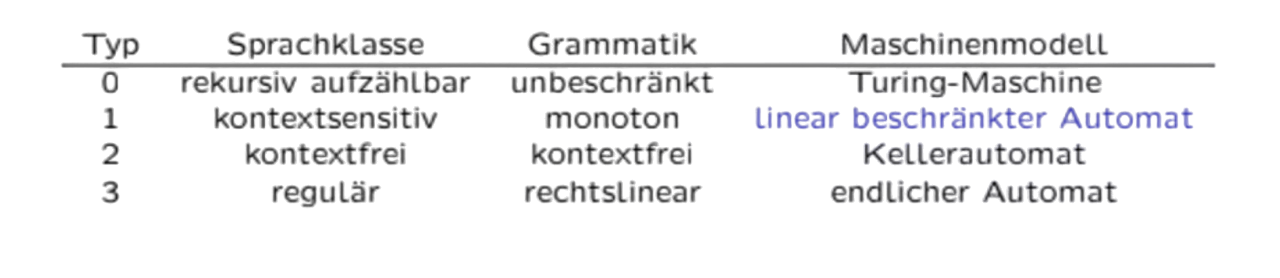
\includegraphics[width=\textwidth]{Bilder/Zusammenhang_Sprache_Grammatik_Maschinenmodell.png}
	
\section{Reguläre Sprachen und endliche Ausdrücke}
	\subsection{Reguläre Ausdrücke}
	Ein regulärer Ausdruck über $\varSigma$ beschreibt eine formale Sprache.\newline
	Die Menge aller regulären Ausdrücke über $\varSigma$ ist eine formale Sprache.\newline\newline
	Beispiel: Sprache aller Wörter über $\varSigma_{abc}$, die nur aus genau zwei Symbolen bestehen:\newline
	Ausdruck: $r_1 = (a + b + c)(a + b + c)$\newline
	Sprache: $\mathcal{L}(r_1) = \{ w \in \varSigma_{abc}^*$ | $|w| = 2\}$\newline
	\noindent Operatoren:
	\begin{center}
		\begin{figure}[!h]
			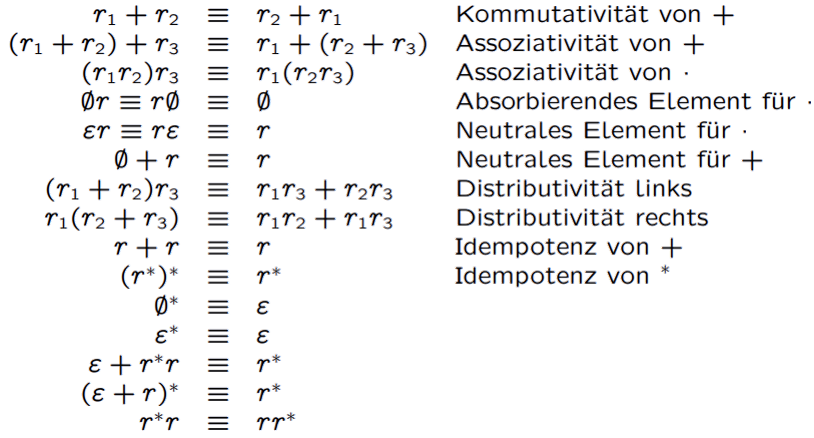
\includegraphics[width=\textwidth]{Bilder/RegulaereAusdruecke_Operatoren.PNG}
		\end{figure}
	\end{center}
	Nicht alle Operatoren sind für alle Typen zulässig:
	\begin{center}
		\begin{figure}[!h]
			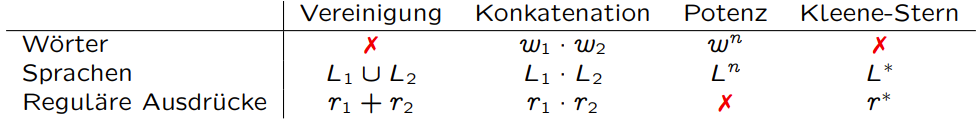
\includegraphics[width=\textwidth]{Bilder/Zulaessige_Operatoren.PNG}
		\end{figure}
	\end{center}

	\subsection{Endliche Automaten}
	Endliche Automaten sind eine andere Darstellung einer regulären Sprache. Endliche Ausdrücke lassen sich in Reguläre Ausdrücke umformen. Genauso auch anders herum.\newline
	Endliche Automaten erkennen regulären Sprachen. Endliche Ausdrücke lassen sich in Reguläre Ausdrücke umformen. Genauso auch anders herum.\newline
	Endliche Automaten lassen sich sowohl deterministisch als auch nicht-deterministisch darstellen.

	\subsubsection{Deterministische endliche Automaten(DEA)}
	Ein DEA hat endlich viele Zustände. Jeder mögliche Übergang muss hierbei behandelt werden können. D.h. für das Alphabet $\varSigma_{ab}$ muss von jedem Zustand sowohl ein $a$, als auch ein $b$ Übergang gegeben sein. Er terminiert wenn das Wort zu ende ist und dabei ein Endzustand erreicht ist.\newline
	\noindent Der DEA lässt sich durch folgendes 5-Tupel darstellen:\newline
	$\mathcal{A} = (Q, \varSigma, \delta, q_0, F)$ mit den Komponenten:\newline
	$Q$ ist eine endliche Menge von Zuständen\newline
	$\varSigma$ ist ein endliches Alphabet\newline
	$\delta: Q \times \varSigma \rightarrow Q$ ist die Übergangsfunktion\newline
	$q_0 \in Q$ ist der Startzustand\newline
	$F \subseteq Q$ ist die Menge der Endzustände\newline
	\newline
	Beispiel:\newline
	\begin{center}
		\begin{figure}[!h]
			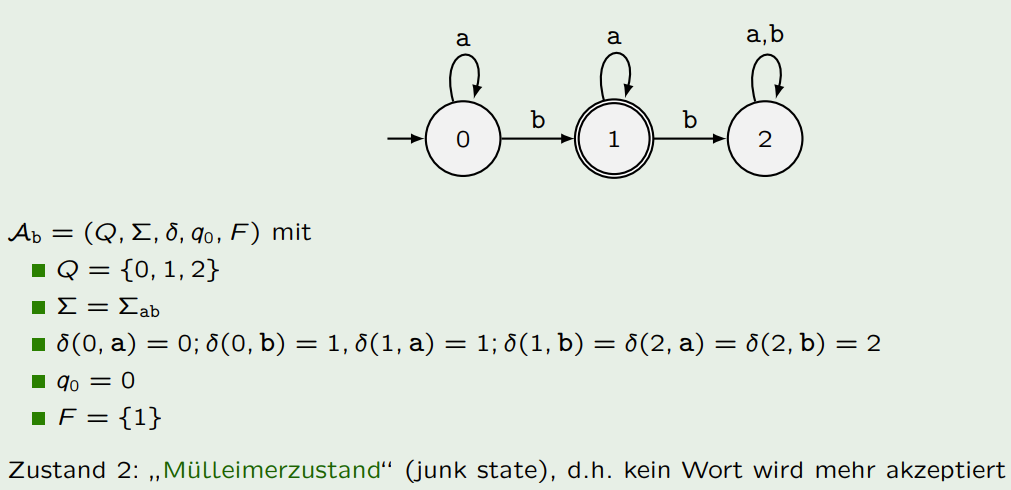
\includegraphics[width=\textwidth]{Bilder/DEA_Beispiel.PNG}
		\end{figure}
	\end{center}
	\textbf{Run/Konfigurationsfolge: } 2er Tupel: (q, w) mit $q \in Q \wedge w \in \sum$*

	\subsubsection{Nicht-deterministische endliche Automaten(NEA)}
	Ein NEA hat endlich viele Zustände. Nicht jeder mögliche Übergang muss hierbei behandelt werden. D.h. für das Alphabet $\varSigma_{ab}$ reicht es, nur den $a$-Übergang, bzw. nur den $b$-Übergang zu besitzen(oder keinen). Der Automat beginnt im Startzustand und muss im Endzustand enden. Wenn der Automat sich nicht in einem Endzustand befindet, befindet sich das Wort nicht in der Sprache, welche vom Automaten abgebildet wird. Zudem gibt es $\varepsilon$-Übergänge, diese können jederzeit verwendet werden ohne ein Eingabesymbol.\newline
	\noindent Der NEA lässt sich durch folgendes 5-Tupel darstellen:\newline
	$\mathcal{A} = (Q, \varSigma, \Delta , q_0, F)$ mit den Komponenten:\newline
	$Q$ ist eine endliche Menge von Zuständen\newline
	$\varSigma$ ist ein endliches Alphabet\newline
	$\Delta$ ist eine Relation über $Q \times (\varSigma \cup \{\varepsilon\}) \times Q$\newline
	$q_0 \in Q$ ist der Startzustand\newline
	$F \subseteq Q$ ist die Menge der Endzustände\newline
	\newline
	Beispiel:\newline
	\begin{center}
		\begin{figure}[!h]
			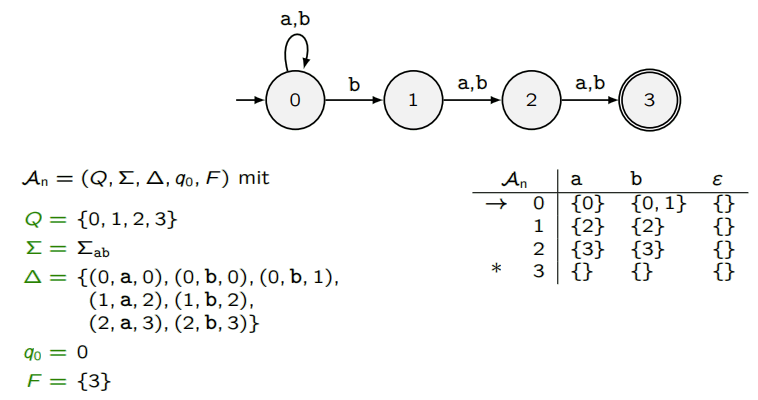
\includegraphics[width=\textwidth]{Bilder/NEA_Beispiel.png}
		\end{figure}
	\end{center}
	\textbf{Run/Konfigurationsfolge: } 2er Tupel: (q, w) mit $q \in Q \wedge w \in \sum$*
	
	\subsubsection{Komplement eines EAs}
	Wird durch vertauschen von End- und Nichtendzuständen erzeugt.

	\subsubsection{Transformation DEA zu RA}
	Um einen DEA zu einem RA umzuformen müssen zuerst die Gleichungen der jeweiligen Zustände aufgestellt und vereinfacht werden:\newline
	\begin{center}
		\begin{figure}[!h]
			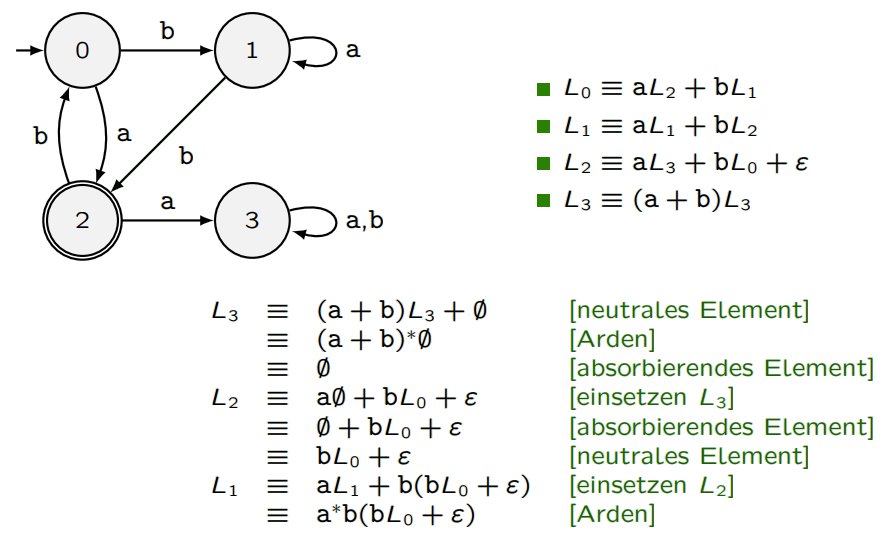
\includegraphics[width=\textwidth]{Bilder/DEAzuRA1.png}
		\end{figure}
	\end{center}
	Da $L_2$ der Endzustand ist, bekommt die Gleichung $\varepsilon$ hinzuaddiert!\newline
	Folglich kann man die gekürzten Gleichungen in einander einsetzen um bis zum Anfangszustand zu kommen:\newline
	\begin{center}
		\begin{figure}[!h]
			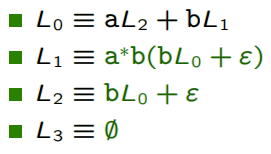
\includegraphics[]{Bilder/DEAzuRA2.png}
		\end{figure}
	\end{center}
	Der vereinfachte Anfangszustand $L_0$ ist dann der RA zum zugehörigen DEA:\newline
	\begin{center}
		\begin{figure}[!h]
			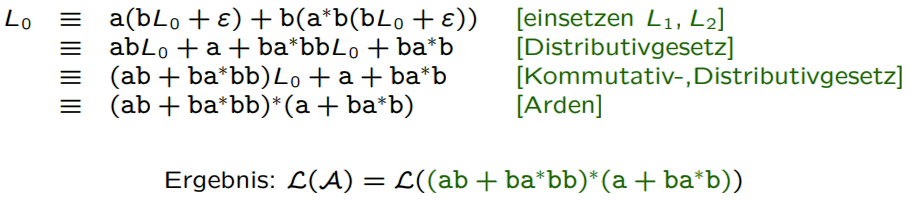
\includegraphics[width=\textwidth]{Bilder/DEAzuRA3.png}
		\end{figure}
	\end{center}

	\subsubsection{RA zu NEA}
	Aus den elementaren RA können einfach NEAs erstellt werden.
	\begin{center}
			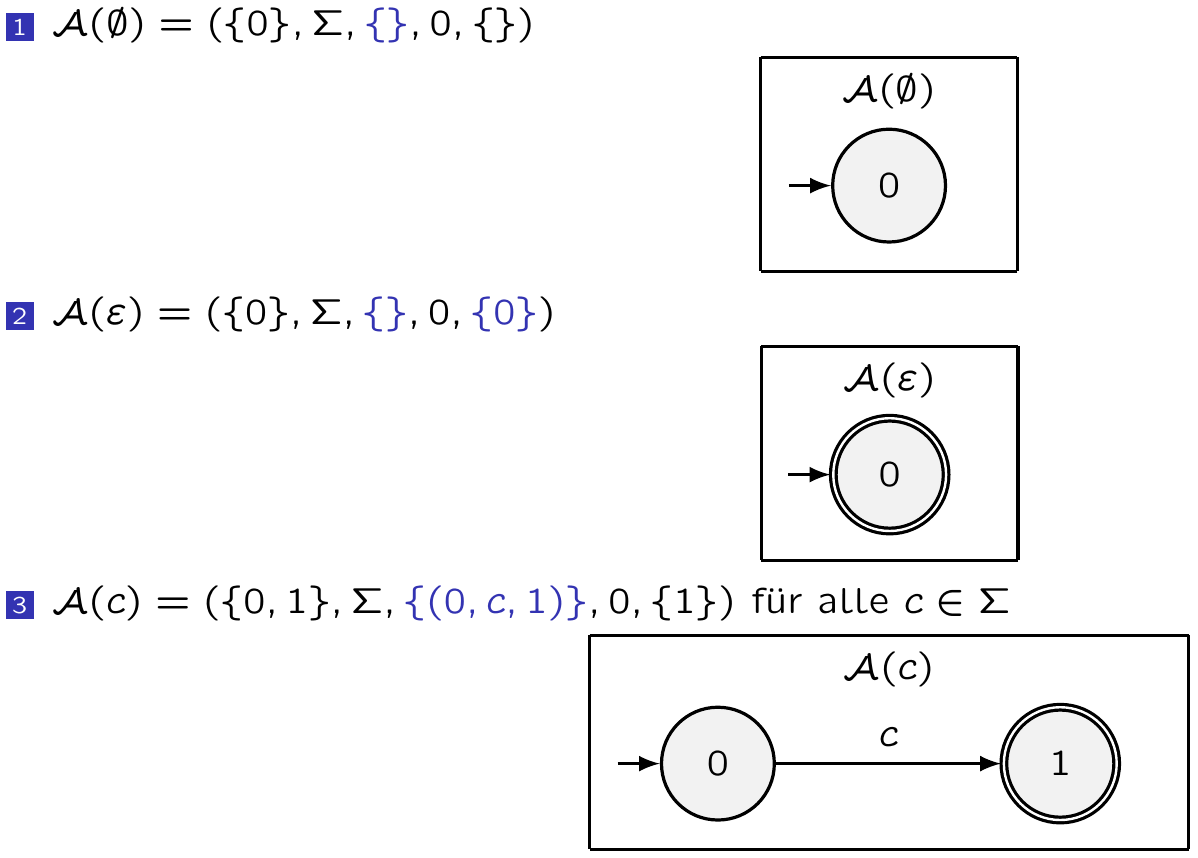
\includegraphics[width=0.8\textwidth]{Bilder/ElementareRAzuDEA.png}
	\end{center}
	Bei komplexen RAs werden die RAs als "BlackBox" dargestellt, dabei werden die Übergänge gepunktet dargestellt.

	\begin{center}
			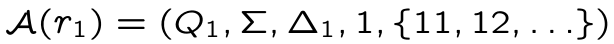
\includegraphics[width=.7\textwidth]{Bilder/KomplexeRABeispiel.png}
	\end{center}

	\begin{center}
			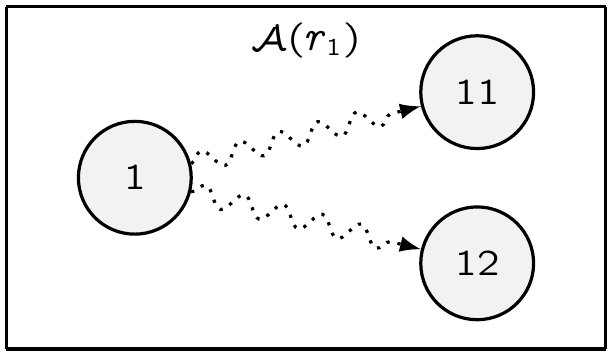
\includegraphics[width=.7\textwidth]{Bilder/BlackBoxExample.png}
	\end{center}

	\begin{center}
			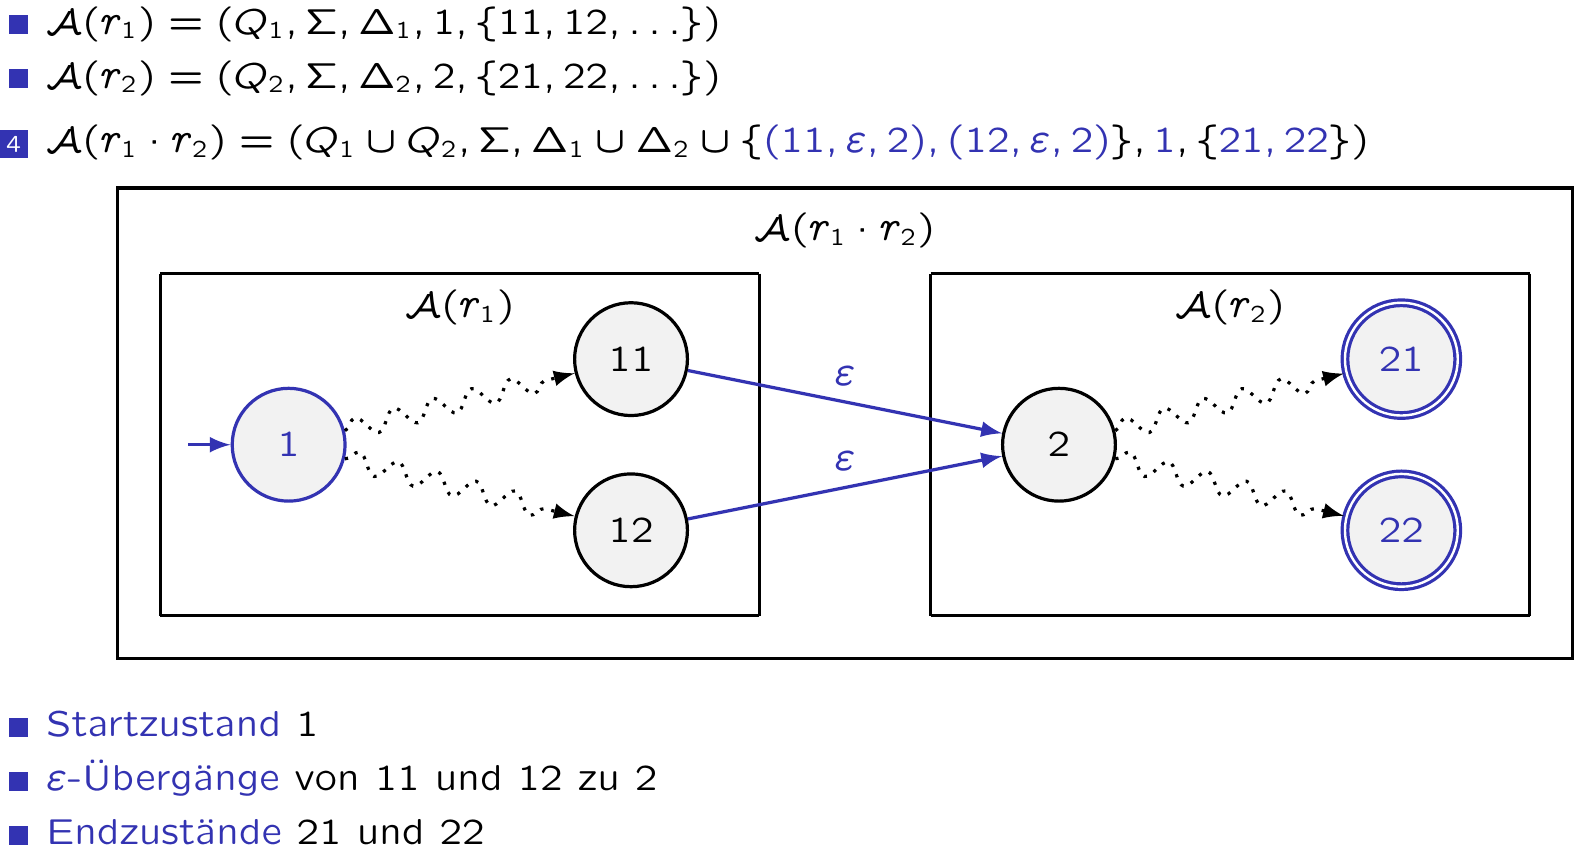
\includegraphics[width=\textwidth]{Bilder/KonkatenationNEA.png}
	\end{center}
	\begin{center}
			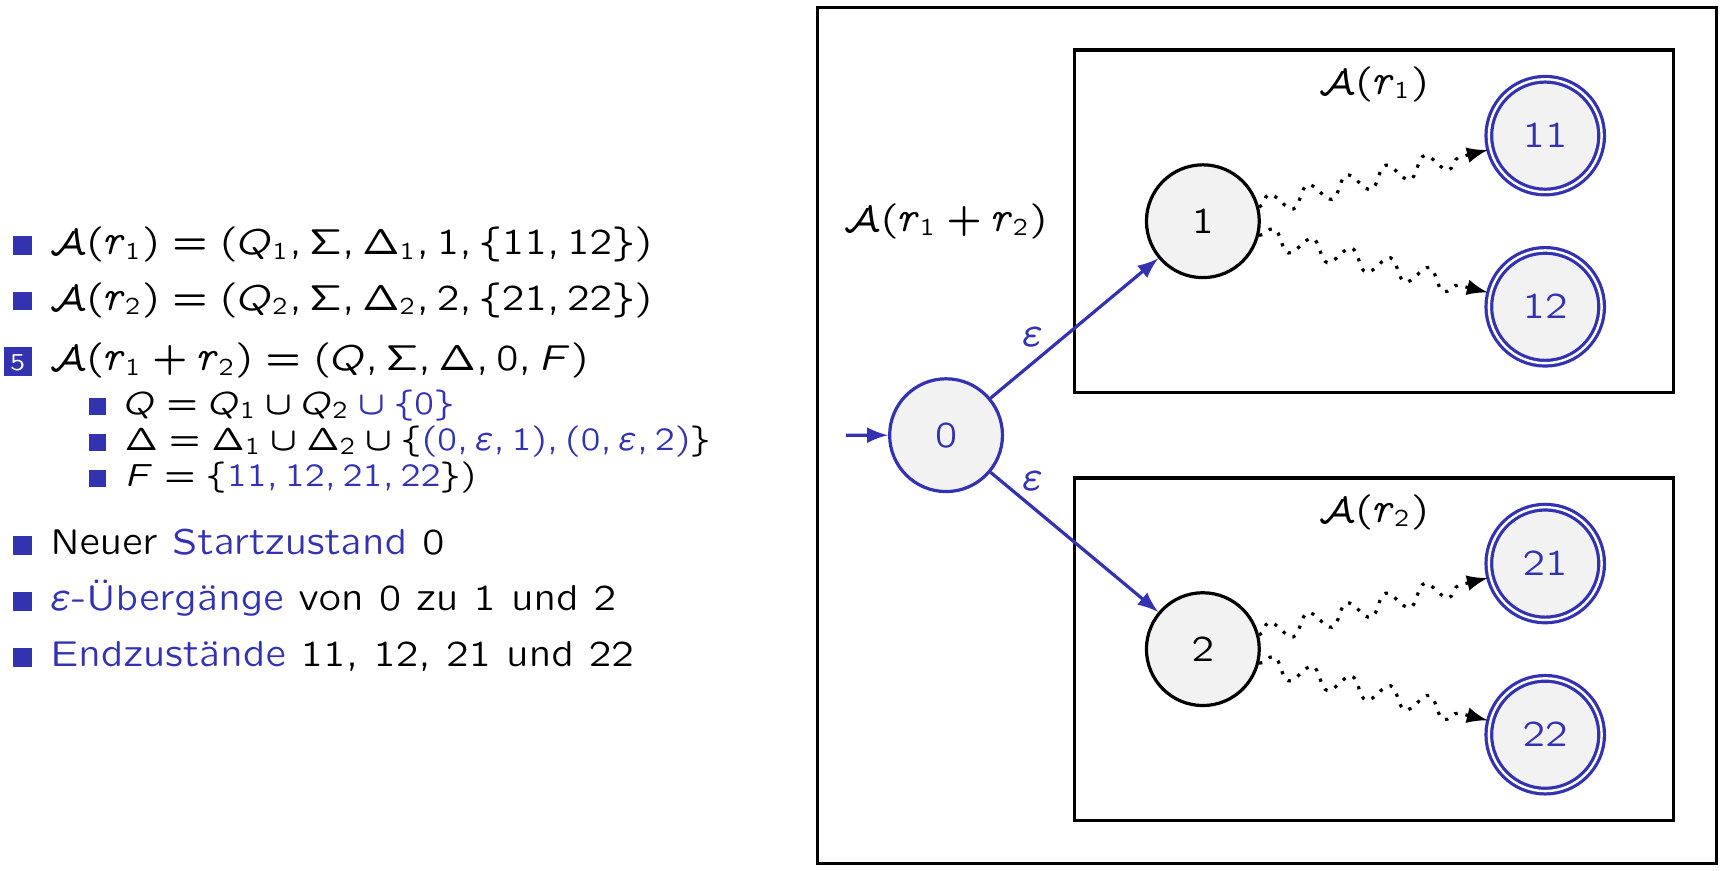
\includegraphics[width=\textwidth]{Bilder/VereinigungNEA.png}
	\end{center}

	\begin{center}
			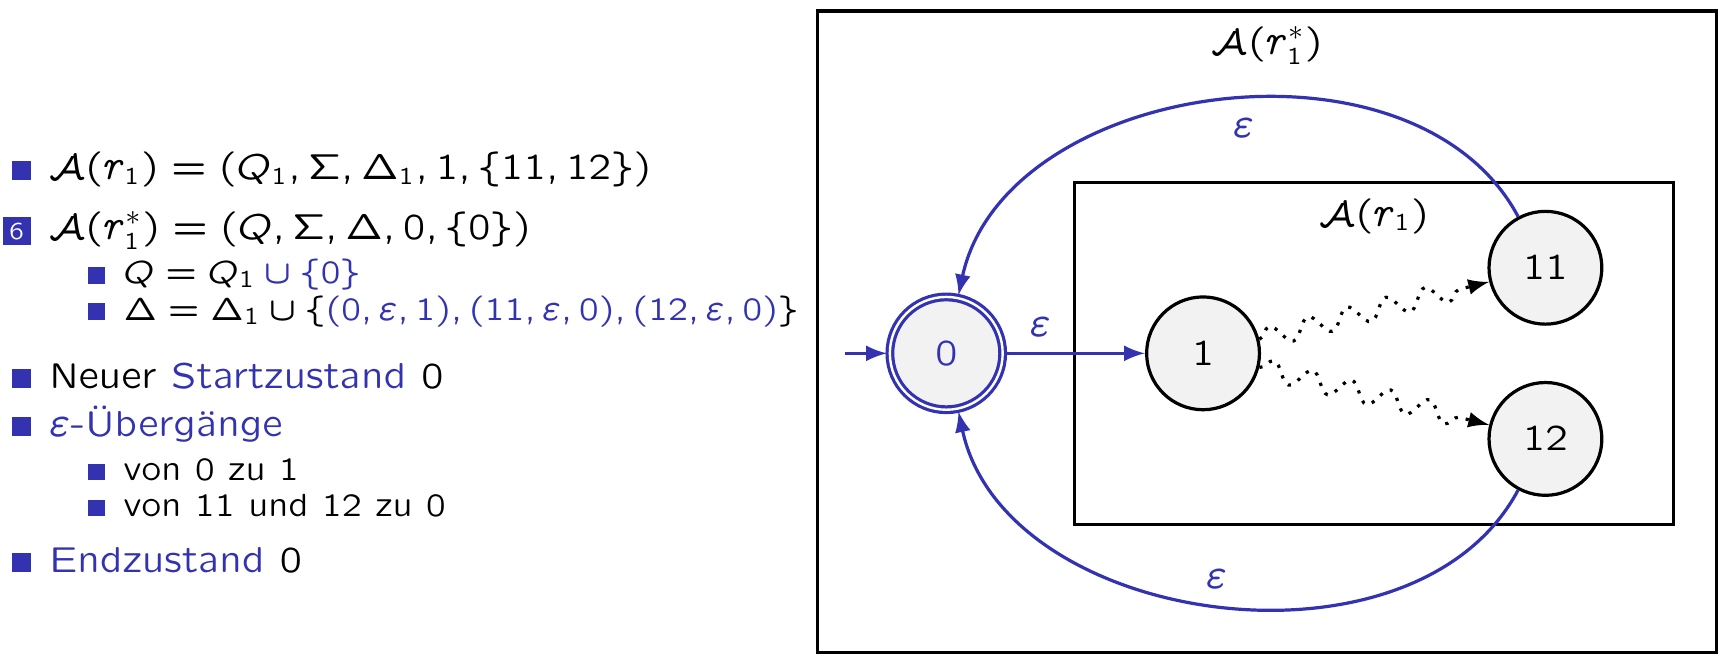
\includegraphics[width=\textwidth]{Bilder/KleeneNEA.png}
	\end{center}

	\newpage

	\subsubsection{NEA zu DEA}
	Zuerst wird eine Transformationstabelle mit neuen Zuständen erstellt. Danach werden die Zustandsmengen als neue Zustände definiert und wenn die Menge einen Endzustand enthält, ist der neue Zustand ein Endzustand.\\\\
	\begin{minipage}[c]{0.5\textwidth}
		\textbf{Übergangstabelle:}\\
		\begin{tabular}[h]{c | c | c}
			& 0 & 1\\
			\hline
			$q_0$ & $\{q_0, q_1\}$ & $q_0$\\
			\hline
			$q_1$ & $\varnothing$ & $q_2$\\
			\hline
			$q_2$* & $\varnothing$ & $\varnothing $
		\end{tabular}
	\end{minipage}
	\hfill
	\begin{minipage}[c]{0.5\textwidth}
		\textbf{Transformationstabelle:}\\
		\begin{tabular}[h]{c | c | c}
			& 0 & 1\\
			\hline
			$q_0$ & $\{q_0, q_1\}$ & $q_0$\\
			\hline
			$\{q_0, q_1\}$ & $\{q_0, q_1\}$ & $\{q_0, q_2\}$*\\
			\hline
			$\{q_0, q_2\}$* & $\{q_0, q_1\}$ & $q_0$
		\end{tabular}\\\\
		$\{q_0, q_1\}$ = p\\
		$\{q_0, q_2\}$* = r
	\end{minipage}
	
	\begin{center}
		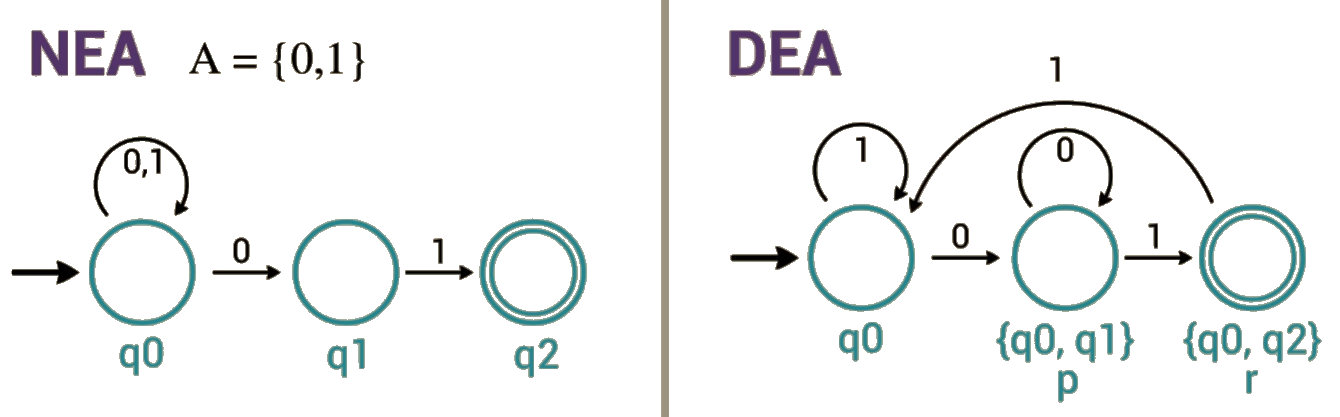
\includegraphics[width=\textwidth]{Bilder/NEAzuDEA.PNG}
	\end{center}

	\subsection{Minimierung}
	Es wird überprüft ob Zustände erreichbar sind, dafür wird vom Startzustand aus jeder Übergang verfolgt und jeder erreichbare Zustand markiert. Alle unmarkierten Zustände können dann einfach aus dem Automaten entfernt werden, da diese Mülleimer Zustände sind. Anschließend muss überprüft werden, ob die Zustände unterscheidbar sind.
	Dafür wird eine Tabelle erstellt, welche alle Zustände beinhaltet. Die Diagonale kann dabei entfernt werden Im Anschluss werden bei den Endzuständen alle nichtendzustände entfernt. Danach müssen die Übergänge getestet werden. Dazu werden für jedes freie Feld in der Tabelle die Übergänge geprüft.\newline
	\begin{center}
			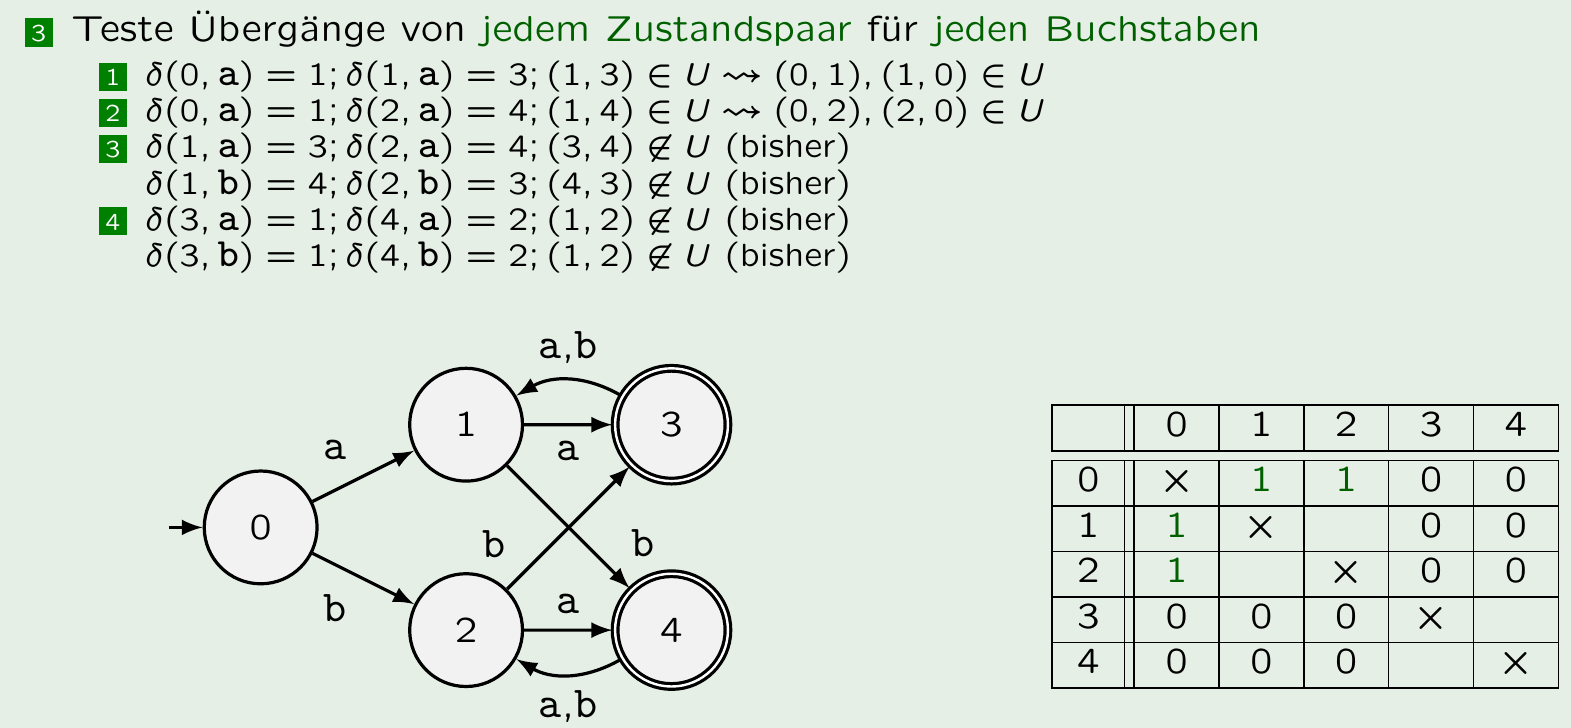
\includegraphics[width=\textwidth]{Bilder/MinimizingUbergangBsp.png}
	\end{center}
	Hier wurden die Übergänge für (1,0),(2,0),(2,1),(4,3) geprüft. Bei (1,0) führt der Übergang a beim Zustand 0 zu 1 und beim Zustand 1 zu 3, (1,3) ist aber schon markiert, deshalb wird in die Zelle eine eins geschrieben. Wenn der Übergang nicht schon markiert wurde kann eine 0 in die Zelle geschrieben werden. \textcolor{red}{Die (Zahl, Zahl) macht kein Sinn oder?}\newline
	\begin{center}
	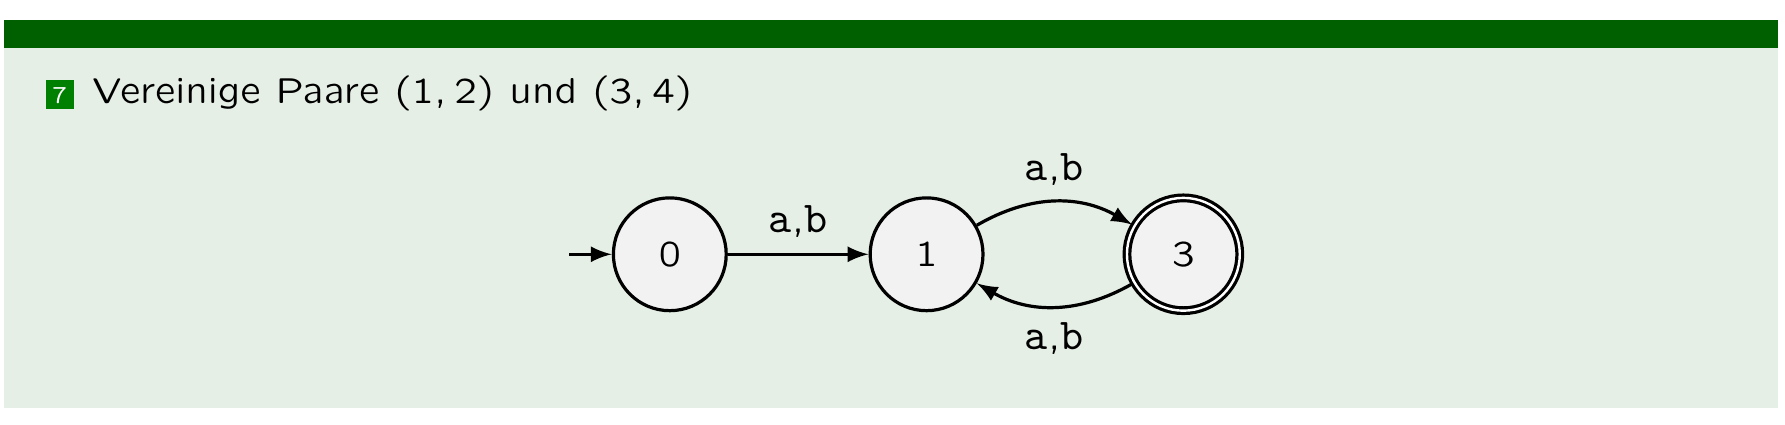
\includegraphics[width=\textwidth]{Bilder/MinimizingVereinigung.png}
	\end{center}
	Die Zustände bei denen eine 1 steht können zusammengefasst werden. Damit ist die Minimierung abgeschlossen.

	\subsection{Nicht-reguläre Sprachen und das Pumping-Lemma}
	\begin{enumerate}
		\item Das gesuchte Wort s besteht aus \textbf{Prolog} u, \textbf{Zyklus} v und \textbf{Epilog} w
		\item Der Zyklus hat mindestest die Länge 1 $v \neq \epsilon$
		\item Prolog und Zyklus zusammen haben höchstens die Länge k
		\item Eine beliebige Anzahl von Zyklus-Durchläufen erzeugt ein Wort der Sprache L
	\end{enumerate}
	\begin{center}
		\begin{figure}[!h]
			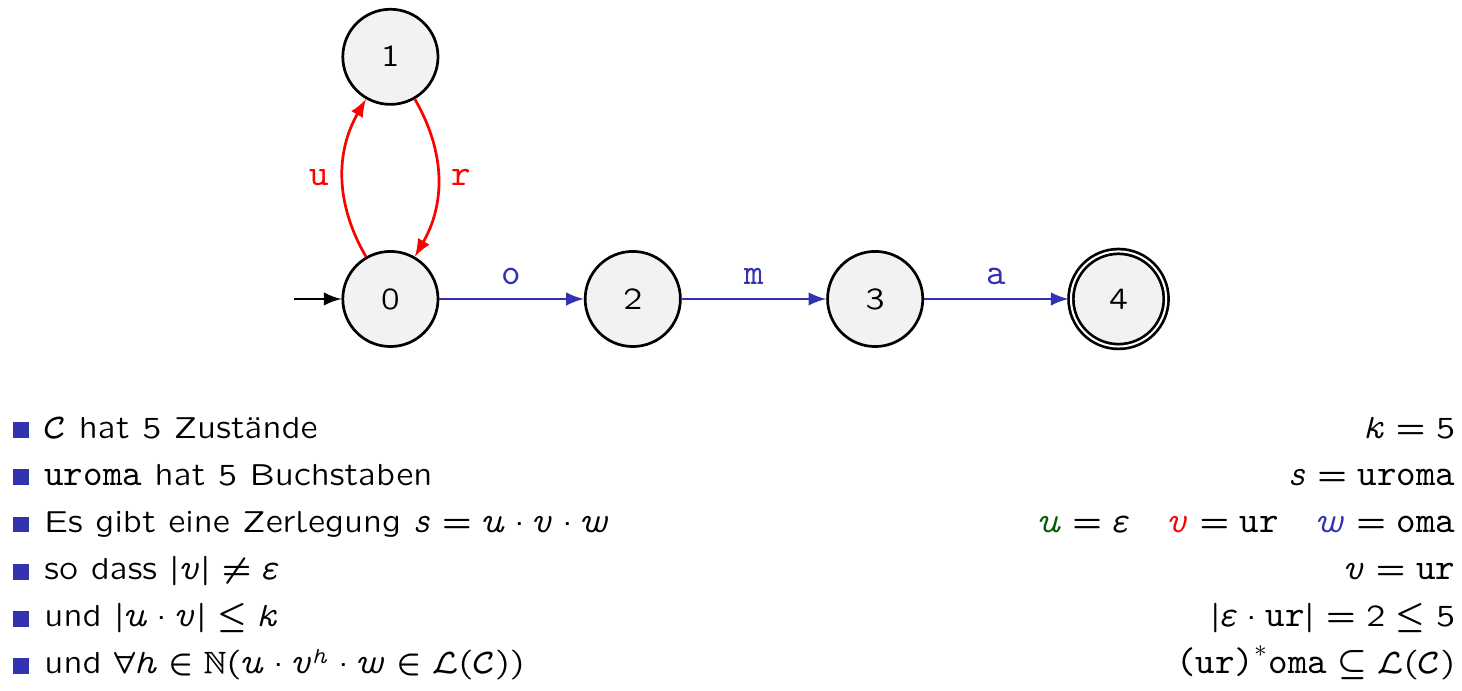
\includegraphics[width=\textwidth]{Bilder/PumpingLemma.png}
		\end{figure}
	\end{center}
	\vspace{.5cm}
	Hier ein Beispiel:
	$$L=\{a^n b^m ~|~ n<m\}$$ \newline
	Das Wort ist damit $a^n b^m$, dieses Word muss in u, v und w aufgeteilt werden um das Pumping Lemma anzuwenden. \newline
	$x = a^nb^{n+1} \in L$ \newline
	$u = a^{n-k}$ \newline
	$v = a^k$ \newline
	$w = b^m$ \newline
	Wir teilen u, v und w so auf, dass wir nun das Pumping Lemma anwenden können, wobei k>0 ist.
	$$x = a^{n-k}(a^k)^ib^{n+1}$$
	Laut dem Pumping Lemma können wir jetzt k beliebig wählen um das erzeugte Wort sollte immer noch ein Teil der Sprache L sein. i steht dabei für die Iterationen, der des Zyklus. \newline
	Also wählen wir $ i = 3$ und Formen die gleichen um.
	$$x = a^{n + k(-1 +3)}b^{n+1}$$
	$$x = a^{n + 2k}b^{n+1}$$
	Weil $k>0$ wissen wir, das das $x \notin L$ und somit auch das L keine reguläre Sprache ist.

	\subsection{Eigenschaften regulärer Sprachen}
	Eine Formale Sprache L ist regulär, wenn es einen \textbf{regulären Ausdruck}, einen \textbf{NEA} oder einen \textbf{DEA} gibt.

	\subsubsection{Leerheitsproblem}
	\begin{enumerate}
	\item Startzustand als erreichbar markieren
	\item Markiere iterativ alle erreichbaren Zustände als erreichbar
	\item Stoppe, wenn ein Endzustand, oder keine neuen erreichbaren Zustände
	\item Falls ein Endzustand erreichbar ist: Ausgabe „nicht leer“
	\item Sonst: Ausgabe „leer“
	\end{enumerate}

	\subsubsection{Wortproblem}
	Man simuliert den Lauf von A auf ein Wort w. Dass heißt man versucht vom Startzustand auf das Wort w zu kommen.

	\subsubsection{Äquivalenzproblem}
	Herausfinden, ob zwei RA's $r_1$ und $r_2$ gleich sind.

	\begin{enumerate}
	\item Zwei NEA's erstellen($A_1, A_2$)
	\item NEA's ind DEA's transformieren($D_1, D_2$)
	\item DEA's Minimieren ($M_1, M_2$)
	\item Zustände von $M_1$ und $M_2$ umbennen.
	\end{enumerate}
	~\newline
	Wenn $M_1 \equiv M_2$ dann gilt auch $r_1 \equiv r_2$

	\subsubsection{Endlichkeitsproblem}
	\begin{enumerate}
		\item Markiere iterativ alle vom Startzustand aus erreichbaren Zustände als erreichbar.
		\item Markiere iterativ alle Zustände, von denen aus ein $q \in F$ erreichbar ist, als terminierend
		\item Sei $A_r$ der Automat, der nur die erreichbaren und terminierenden Zustände von A enthält (gleiche Übergänge)
	\end{enumerate}
	~\newline
	Ist $A_r$ zyklisch folgt, dass $\mathcal{L}(A)$ unendlich ist 

	\subsubsection{Produktautomaten}
	Kreuzprodukt der Zustände von $A_1$ und $A_2$ erstellen. \newline
	Für jeden Zustand die dazugehörigen Übergänge betrachten.\newline
	Dabei wird zum Beispiel für den Zustand $(z_0, q_0)$ überprüft zu welchem Zustand der Übergang 1 führt. Der Zustand $z_0$ führt mit dem Übergang 1 zum Zustand $z_1$ und $q_0$ zu $q_1$, dass heißt das der Zustand $(z_0, q_0)$ mit dem Übergang 1 zum Zustand $(z_1, q_1)$ führt.\newline
	\begin{center}
		\begin{figure}[!h]
			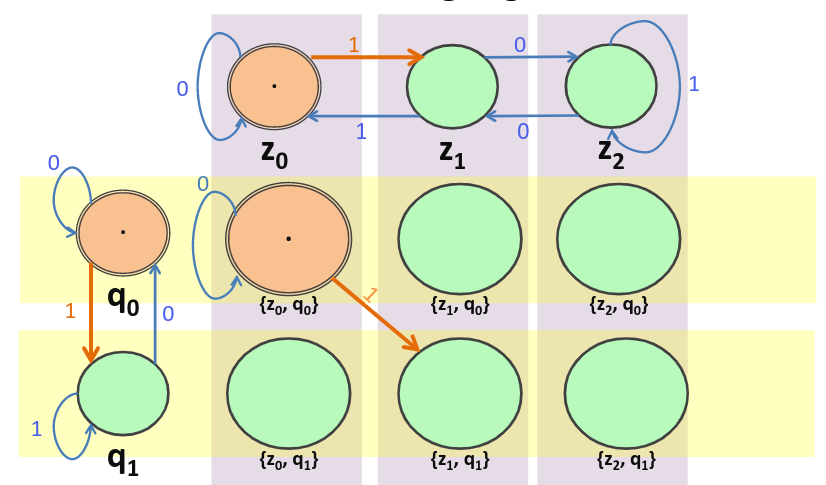
\includegraphics[width=\textwidth]{Bilder/ProduktautomatUbergang.png}
		\end{figure}
	\end{center}


\section{Chomsky Grammatiken und kontextfreie Sprachen}
	Gramatiken erzeugen formale Sprachen dar.\\
	G=($N, \sum , P, S$) mit:\\
	\begin{description}
		\item[N] Nichtterminalsymbole. Diese können für Regeln verwendet werden, aber dürfen nicht selbst im abgeleiteten Wort stehen.
		\item[P] Ableitungsregeln. Bsp.: P=$\{ S \rightarrow Aa | \varepsilon , A \rightarrow a \} $ 
		\item[S] Startsymbol (ist nichtterminel)
	\end{description}

	\subsection{Chomsky-Hierarchie}
	\subsubsection{Typ0 unbeschränkt}
	Ja oke?

    \subsubsection{Typ1 Monoton}
    $\alpha \rightarrow \beta$ mit $| \alpha | \leq  | \beta |$ und Ausnahme $S \rightarrow \varepsilon$, wenn S auf keiner rechten Seite ist.

    \subsubsection{Typ2 Kontextfreie}
	A $\rightarrow \beta$ mit A $\in$ N und $\beta \in V$* 

    \subsubsection{Typ3 Rechtsregulär/-linear (RLG)}
	A $\rightarrow$ cB mit A $\in$ N; B $\in$ N $\cup$ $\{ \varepsilon \}$; c $\in \sum \cup \{ \varepsilon \}$

	\subsubsection{DEA zu RLG}
	\textbf{A} = (Q, $\sum$, $\delta$, $q_0$, F) $\Rightarrow$ \textbf{G} = (N, $\sum$, P, S)\\
	mit: \textbf{N} = Q, \textbf{S} = $q_0$ und \textbf{P} = $\{p \rightarrow cq | \delta (p, c) = q\} \cup \{p \rightarrow \epsilon | p \in F\}$ \\
	Bsp.: Kommt man mit a von Zustand 0 zu Endzustand 1: P=$\{ 0 \rightarrow a1, 1 \rightarrow \epsilon \}$

	\subsubsection{RLG zu NEA}
	\textbf{G} = (N, $\sum$, P, S) $\Rightarrow$ \textbf{A} = (Q, $\sum$, $\delta$, $q_0$, F)  \\
	mit: \textbf{Q} = N $\cup\{f \; | f \notin N\}$, \textbf{F} = $\{f\}$, $q_0$ = S und\\
	$\Delta$ = $\{ (A, c, B) | A \rightarrow cB \in P\} \cup \\
	\{ (A, c, f) | A \rightarrow c \in P\} \cup \\
	\{ (A, \epsilon, B) | A \rightarrow B \in P\} \cup \\ 
	\{ (A, \epsilon, f) | A \rightarrow \epsilon \in P\}$
	Prinzip: Regeln umwandeln und Endzustände $f$ hinzufügen.

	\subsubsection{Kellerautomaten}
	Endlicher Automat mit unendlichem Stack, auf welchem nur der oberste/neueste Buchstabe gelesen, ">gepusht"< oder ">gepopt"< werden kann.\\
	\textbf{Akzeptanzbedingung: } Leerer Stack und Wort zu Ende.\\
	\textbf{Deterministisch, } wenn in jeder Konfiguration nur eine Folgkonfiguration möglich ist.\\
	\textbf{Syntax:} A=(Q, $\Sigma$, $\Gamma$, $\Delta$, $q_0$, Z)\\\\
	\begin{minipage}[c]{0.5\textwidth}
		\begin{description}
			\item[Q] Zustände
			\item[$\sum$] Alphabet
			\item[$\Gamma$] Stack-Alphabet
			\item[$q_0$] Startzustand
			\item[Z] Startstacksymbol  
			\item[$\Delta$] Regeln in Tabellenform $\Rightarrow$
		\end{description}
		Im Graph $\Delta$-Regeln ohne Zustände angeben:
	\end{minipage}
	\begin{minipage}[c]{0.5\textwidth}
		$\Delta$\textbf{-Bsp.:}\\
		\begin{tabular}[h]{c|c|c|c|c}
			Q & $\sum$ & $\Gamma$ & $\Gamma$* & Q\\
			\hline
			(0, & a, & A, & AA, & 0)\\
			(0, & b, & A, & $\epsilon$, & 1)\\
			&&...
		\end{tabular}
		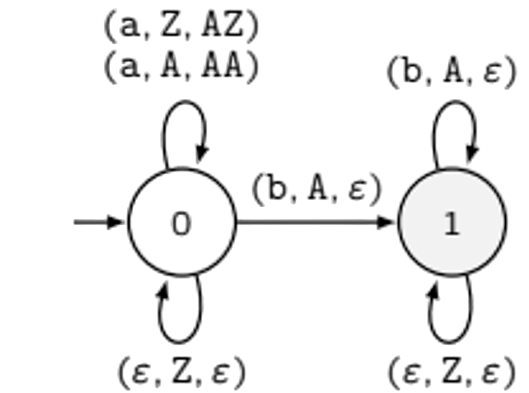
\includegraphics[scale=0.3]{Bilder/KellerAutomat.png}
	\end{minipage}
	\textbf{Run/Konfigurationsfolge:} 3er Tupel: (q, [Stack], Wort)

	\subsection{Cocke-Younger-Kasami(CYK)-Algorythmus}
	Entscheidet Wortproblem für kontextfreie Grammatiken in CNF. Bsp.:\\
	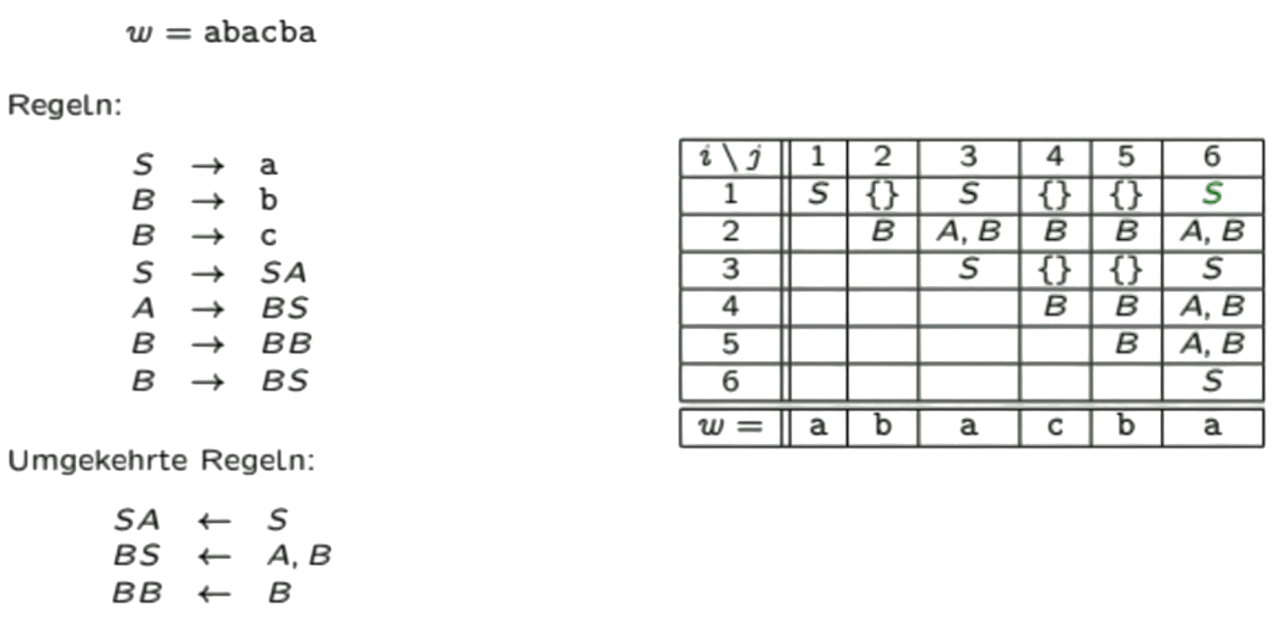
\includegraphics[scale=0.3]{Bilder/cyk-Algo.png}
	\begin{enumerate}
		\item Wort unter Tabelle schreiben 
		\item Umgekehrte Regeln bilden (optional)
		\item Herleitungen in Tabellen-Diagonale eintragen
		\item Herleitungen der Teilwörter als Menge eintragen (alle Möglichkeiten)
	\end{enumerate}

	\subsection{Chomskynormalform CNF}
	Zur Entscheidung des Wortproblems. Nur Regeln mit Syntax: \\
	1. $A \rightarrow BC$ oder 2. $A \rightarrow a$ mit $A,B,C \in Nichtterminalsymbole \; \wedge \; a \in Terminalsymbole$ und $S \rightarrow \epsilon$, wenn S auf keiner Rechten Seite ist.\\
	\textbf{Vorgehen:}
	\begin{enumerate}
		\item Epsilon-Regeln entfernen
		\begin{enumerate}
			\item Erstelle Liste L mit $A\rightarrow \epsilon$-Regeln und allen Regeln, die auf Nichtterminalsymbole in L zeigen.
			\item Ergänze rechte Seite der Regeln mit sich selbst mit eingesetztem $\epsilon$ für Nichtterminalsymbole $\in$ L
			\item Wenn $S \in L$ füge Regel $S_0 \rightarrow S | \epsilon$ ein
		\end{enumerate}
		\item Kettenregel entfernen
		\begin{enumerate}
			\item Erstelle Listen für Kettenregeln ausgehend von jeweiligen Nichtterminalen
			\item Ergänze Regeln mit allen Kettenregeln
			\item Regeln kürzen
		\end{enumerate}
		\item überflüssige Symbole entfernen
		\item Einzelne Nichtterminalsymbole auf rechter Seite ersetzen 
		\item Rechte Seite mit Hilfssymbolen kürzen
	\end{enumerate}
	
	\subsection{Eigenschaften kontextfreier Sprachen}
	
	\textbf{Pumping-Lemma 2}\newline
	Für jedes $s \in L$ mit $|s| \geq k$ gibt es eine Zerlegung $s = u*v *w*x*y$
	
	\begin{enumerate}
	\item $vx \neq \epsilon$
	\item $|vwx| \leq k$
	\item $u*v^h*w*x^h*y \in L $ für alle $h \in \mathbb{N}$
	\end{enumerate}
Wie im normalen Pumping Lemma wird ein Wort der Sprache in teile aufgespalten, wobei v und x aufgepumpt werden, um zu zeigen, dass sie die Regeln der Sprache verletzen, wodurch gezeigt wird, dass die Sprache nicht kontextfrei ist.\newline
Mit einer kontextfreien Sprache können Vereinigungen, Konkatenation und Kleene-Stern verwendet werden. Durchschnitt und Komplement aber nicht.\\
Das Aquivialenzporoblme ist aber unentscheidbar.´
	

\section{Turing Maschine}
	\subsection{Turing Maschine mit einem endlosem Einleseband}
	Terminiert wenn Endzustand erreicht und Einleseband nicht verschiebbar ist.\\
	M=(Q, $\sum, \Gamma , \Delta , q_0$, F) mit:\\
	\begin{description}
		\item[$\Gamma$] Vereinigung aus mindestens Blank-Symbol und Terminalsymbole: $\Gamma \supseteq \sum \cup \{ \square \} $
		\item[$\Delta$] Übergangsrelationen Syntax: IST-Zustand IST-Inhalt Neuer-Inhalt Verschiebung Neuer-Zustand Bsp.: $0 \left( \begin{array}{c} a \\ \square \end{array}\right) \left( \begin{array}{c} a \\ a \end{array}\right) \left( \begin{array}{c} r \\ l \end{array} \right) 1$
		\item[F] Endzustände
	\end{description}
	\textbf{Run/Konfigurationsfolge:} startet mit "> $q_0$w "<, mit w $\in \sum$* und akzeptiert, wenn "> $q \Box $ "< , mit $q \in Q$ 

	\begin{center}
	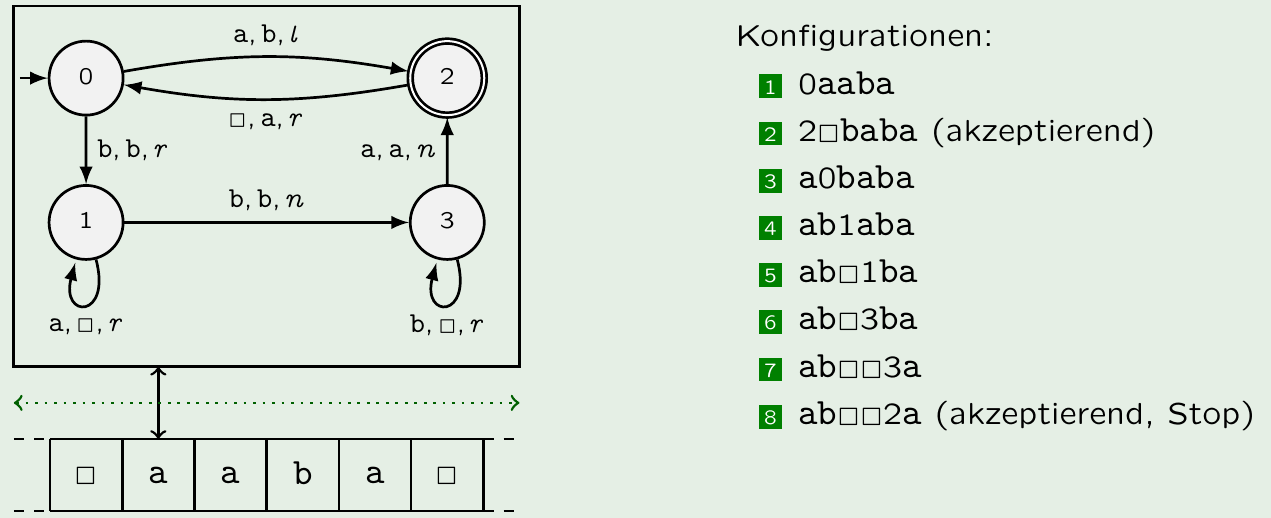
\includegraphics[width=\textwidth]{Bilder/Turing.png}
	\end{center}
	
	\subsection{Mehrband-Turingmaschine}
	
	Wie eine normale Turingmaschine, mit dem Unterschied, dass es mehere Bänder gibt.
	\begin{center}
		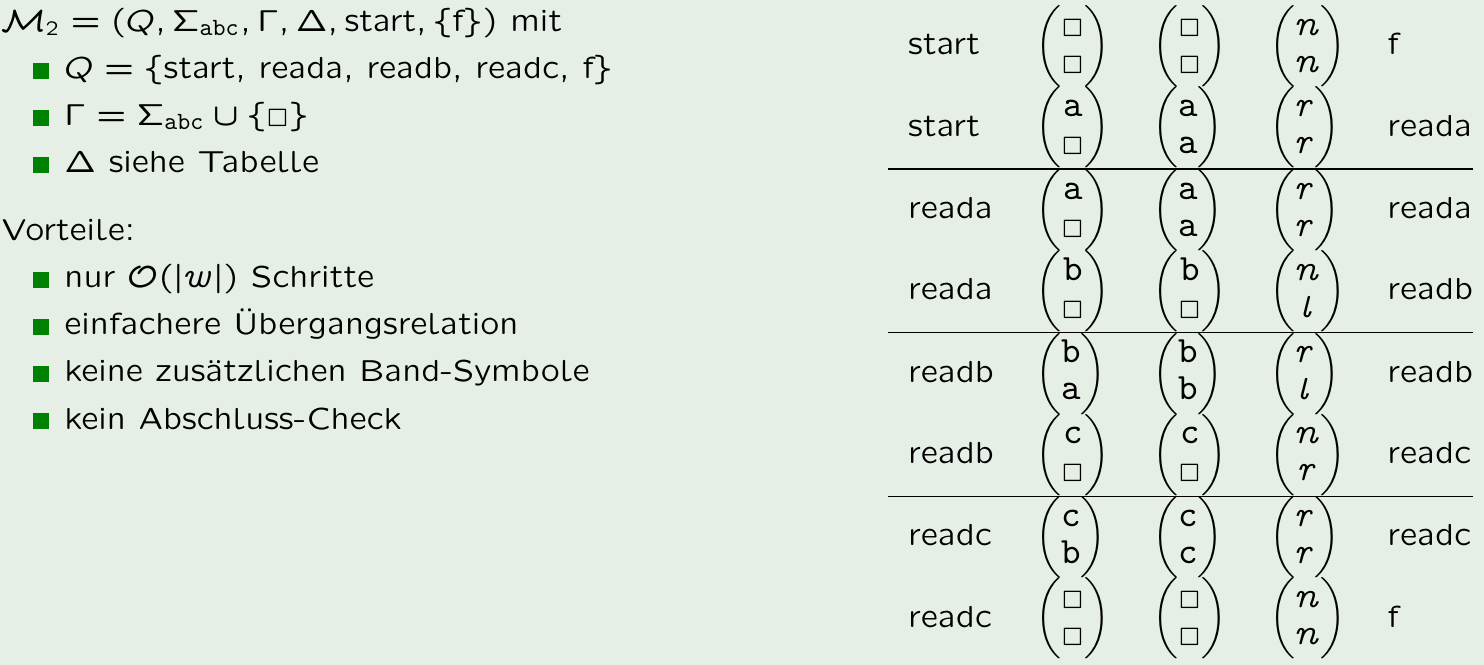
\includegraphics[width=\textwidth]{Bilder/MehrbandTuring.png}
	\end{center}
Die Maschinenmodelle „Turing-Maschine“ und „ k-Band-Turing-Maschine“ sind äquivalent.\newline
	
	\begin{itemize}
	\item Nichtdeterministische Turingmaschinen
	\begin{itemize}
	\item können durch eine deterministische 2-Band-TM simuliert werden
	\item beschreiben dieselbe Sprachklasse wie 1-Band-Turingmaschinen
	\end{itemize}
	\end{itemize}

	\subsection{Unbeschränkte Grammatiken}

	\begin{center}
	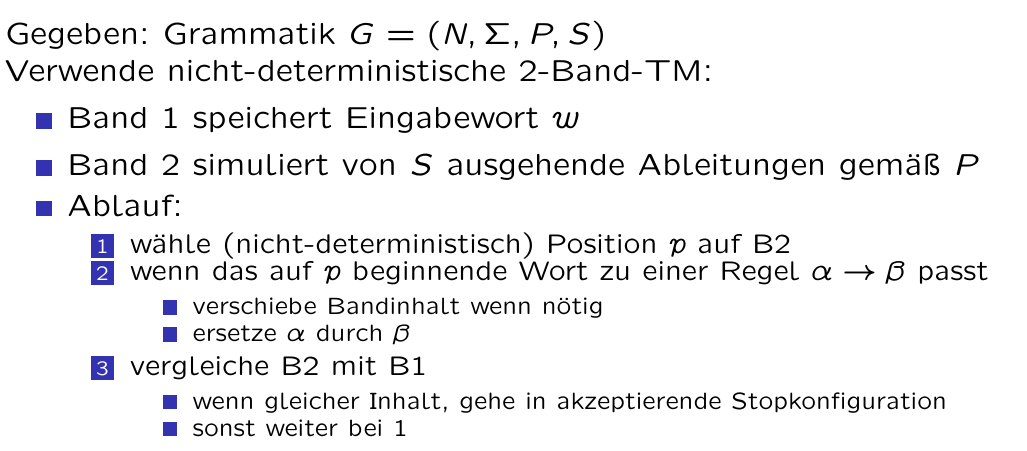
\includegraphics[width=\textwidth]{Bilder/Typ0Grammatik.png}
	\end{center}

	\subsection{Linear beschränkter Automat}
		Touring Automat mit beschränktem Band durch Start- und Endsymbol (Band: " $>abaab<$ ")


\section{Entscheidbarkeit}
	\subsection{Unentscheidbarkeit des speziellen Wortproblems}

	\subsection{Reduktionsweise}
	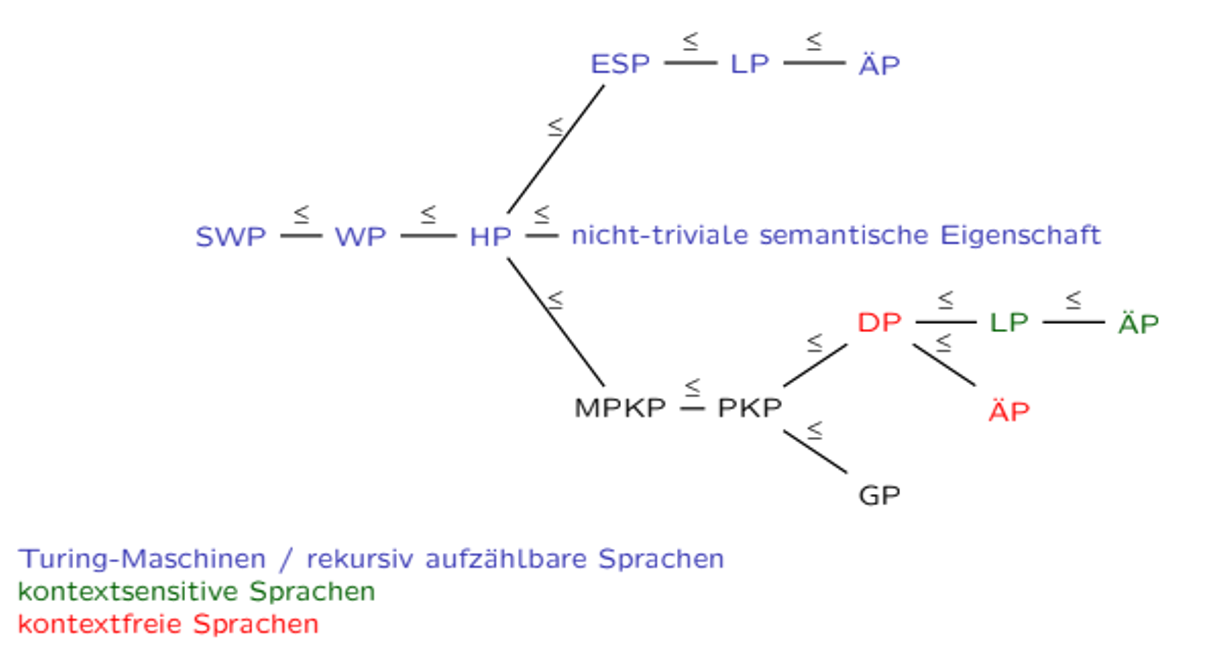
\includegraphics[scale=0.4]{Bilder/Zusammenfassung_Unentscheidbarkeiten.png}

	\subsection{Das PKP und weitere unentscheidbare Probleme}
	Endliche Folge an Wortpaaren, mit nichtleeren Wörtern, über endlichem Alphabet.\\
	\textbf{Syntax:} P=($(l_1, r_1), (l_2, r_2), ...(l_n, r_n)$) \hfill \textbf{Lösung:} $l_{i_1} \cdot l_{i_2} \cdot ... \cdot l_{i_n} = r_{i_1} \cdot r_{i_2} \cdot ... \cdot r_{i_n}$

	\subsection{Semi-Entscheidbarkeit}
	
	\subsection{Die universelle Turingmaschine}

	\subsection{Abschlusseigenschaften}

\section{Berechenbarkeit}
	\subsection{Turing Berechenbarkeit}

	\subsection{WHILE Programme}

	\subsection{Die Church-Turing-These}

\section{Komplexität}
	\subsection{Komplexitätsklassen}

	\subsection{NP-Vollständigkeit}

\end{document}